%% This LaTeX-file was created by <karsten> Thu Feb 11 22:25:30 1999
%% LyX 1.0 (C) 1995-1999 by Matthias Ettrich and the LyX Team

%% Do not edit this file unless you know what you are doing.
\documentclass[12pt,a4paper,oneside]{book}
\usepackage[T1]{fontenc}
\usepackage{palatino}

\makeatletter


%%%%%%%%%%%%%%%%%%%%%%%%%%%%%% LyX specific LaTeX commands.
\newcommand{\LyX}{L\kern-.1667em\lower.25em\hbox{Y}\kern-.125emX\@}
\newcommand{\noun}[1]{\textsc{#1}}

%%%%%%%%%%%%%%%%%%%%%%%%%%%%%% User specified LaTeX commands.
\usepackage{html, epsfig}
\makeatletter
\makeatother

\begin{document}


\vfill{}
\title{\textit{M}\\
User Manual}
\vfill{}


\author{Copyright 1999 by Karsten Ball�der <\texttt{Ballueder@usa.net}>\\
Written by Karsten Ball�der and Vadim Zeitlin}

\maketitle
\tableofcontents


\chapter{Using M }


\section{Release Notes}

Some quick notes about this release of M.


\subsection{WARNING - this is alpha}

When you do a large free software project, you have two choices: either continue
hacking without releases and risk to never get it finished, or set yourself
a release date, no matter what the situation is. As we got several requests
from people who want to play with it, we decided on a release date and did our
best to get it into a working shape. BUT THIS SOFTWARE IS STILL UNDER DEVELOPMENT!
This means

\begin{itemize}
\item it is incomplete and may be awkward to use
\item it may crash occasionally or often or be completely unusable - \textit{Use it
at your own risk!}
\end{itemize}

\subsection{Which features are implemented?}

Quite some already, but more are still missing. What we have so far:

\begin{itemize}
\item Cross-platform. M compiles on a variety of Unix systems and on Microsoft Windows.
Use one mail client, no matter what system you use. The source and binary for
Windows 95/98/NT are available on request (\htmladdnormallink{\texttt{m-developers@makelist.com}}{\texttt{m-developers@makelist.com}}).
Mailbox file formats are the same on both platforms.
\item Based on the c-client library from the University of Washington, therefore full
access to a wide range of protocols and file formats, including SMTP, MAP, POP3,
NNTP and several mailbox formats.
\item Wide (extreme?) user configurability. Whatever makes sense to override or change,
can be changed by the user. Configuration supports several configuration files
on Unix, with special administrator support for making entries immutable, and
the registry on Windows.
\item Scriptable and extendable. M includes an embedded Python interpreter with full
access to its object hierarchy. Write object-oriented scripts to extend and
control M.
\item Easy MIME support. Text and other content can be freely mixed and different
filetypes are represented by icons.
\item Inline displaying of images, clickable URLs, XFace support.
\item Multiple mail folders, basic news support.
\item Powerful address database and contact manager 
\item Printing of nicely formatted messages.
\item Full internationalisation support, M speaks multiple languages, but no complete
translations yet.
\end{itemize}

\subsection{Known bugs}

\begin{itemize}
\item some
\end{itemize}

\subsection{TODO, features to implement}

This is a list of features on our TODO list that we are currently working on.
It is not necessarily up to date or complete.

\begin{itemize}
\item add keyboard accelerators
\item Better Python support. We have some callbacks in place, but after the class
hierarchy rewrite we have to generate new interface files for the complete class
hierarchy. Also by this time wxPython might be integrated, so we can actually
write some of the configuration dialogs in python which should speed things
up. \textit{Help welcome.}
\item Full Drag and Drop interaction with filemanagers of Windows and Gnome (will
be added real soon, easy).
\item Clipboard support
\item Easy to use filtering system for mails.
\item Support for V-cards.
\item Nested mail folder hierarchy.
\item Spam-Ex spam fighting/auto-complaint function.
\item Rich-text editing and HTML mail support
\item Support for PGP and GNU Privacy Guard to encrypt mails.
\item Threading of messages and proper usenet news support.
\item Compression of mail folders.
\item Delay-Folder to keep mails and re-present them at a later date.
\item Context sensitive help system (HTML based).
\item Translations to German, French and Italian.
\item Wide character (Unicode) support and other character sets.
\item More import, export and synchronisation with other programs' address databases.
\item Voice mail.
\item More Python support through wxPython.
\item Support for Drag and Drop interaction with KDE, once that wxQt is available.
\item CORBA support, possible cooperation with PINN project.
\item ANY OTHER SUGGESTION
\end{itemize}

\subsection{Help Needed}

As you can see, we have big plans for M. To achieve all this, we need some help.
Areas where we would use some help are

\begin{itemize}
\item Python 
\item support for further mail protocols, LDAP
\item The wxQt project, a port of wxWindows to the Qt toolkit, will also be happy
for any help. We are not directly involved in this, but being involved with
wxWindows, we are happy to support that port.
\item If you have access to other systems apart from Linux/Solaris/Windows, you are
very welcome to help us port M to those platforms, or to other hardware than
Intel.
\end{itemize}

\subsection{Copyright}

M is copyright by Karsten Ball�der and Vadim Zeitlin. It is licensed under the
M ``Artistic License'' as stated in section\ref{License}. Some part of the
source tree distributed with M is not covered under this license. These additional
sources can be found in the ``\texttt{extra/src}'' subdirectory. Please check
the files in the individual directories for their copyright notices. However,
they can freely distributed under certain conditions.


\subsection{The M ``Artistic License''\label{License}}


\subsubsection{Preamble}

The intent of this document is to state the conditions under which this software
package may be copied, such that the Copyright Holder maintains some semblance
of artistic control over the development of the package, while giving the users
of the package the right to use and distribute the Package in a more-or-less
customary fashion, plus the right to make reasonable modifications. 

This license is based on Perl's ``Artistic License'' and has been adapted to
better suit M. It aims to confirm with the Open-Source specification.


\subsubsection{Definitions}

``Package'' refers to the collection of files distributed by the Copyright Holder,
and derivatives of that collection of files created through textual modification. 

``Standard Version'' refers to such a Package if it has not been modified, or
has been modified in accordance with the wishes of the Copyright Holder as specified
below. 

``Copyright Holder'' is whoever is named in the copyright or copyrights for
the package. 

``You'' is you, if you're thinking about copying or distributing this Package. 

``Reasonable copying fee'' is whatever you can justify on the basis of media
cost, duplication charges, time of people involved, and so on. (You will not
be required to justify it to the Copyright Holder, but only to the computing
community at large as a market that must bear the fee.) 

``Freely Available'' means that no fee is charged for the item itself, though
there may be fees involved in handling the item. It also means that recipients
of the item may redistribute it under the same conditions they received it. 


\paragraph{Conditions of Use}

\begin{enumerate}
\item You may make and give away verbatim copies of the source form of the Standard
Version of this Package without restriction, provided that you duplicate all
of the original copyright notices and associated disclaimers and only distribute
the complete package as a whole. 
\item You may apply bug fixes, portability fixes and other modifications derived from
the Public Domain or from the Copyright Holder. A Package modified in such a
way shall still be considered the Standard Version. 
\item You may otherwise modify your copy of this Package in any way, provided that
you insert a prominent notice in each changed file stating how and when you
changed that file, and provided that you do at least ONE of the following: 

\begin{enumerate}
\item place your modifications in the Public Domain or otherwise make them Freely
Available, such as by posting said modifications to Usenet or an equivalent
medium, or placing the modifications on a major archive site such as sunsite.unc.edu,
or by allowing the Copyright Holder to include your modifications in the Standard
Version of the Package, and rename any non-standard executables so the names
do not conflict with standard executables, which must also be provided, and
provide a separate manual page for each non-standard executable that clearly
documents how it differs from the Standard Version. You must not make the modified
version depend on any other software or libary if that software or libary is
not Freely Available or if it is covered under a license more restrictive than
this. 
\item use the modified Package only within your corporation or organization. c.make
other distribution arrangements with the Copyright Holder. 
\end{enumerate}
\item You may distribute the programs of this Package in object code or executable
form, provided that you do at least ONE of the following: 

\begin{enumerate}
\item distribute a Standard Version of the executables and library files, together
with instructions (in the manual page or equivalent) on where to get the Standard
Version. 
\item accompany the distribution with the machine-readable source of the Package with
your modifications, including the complete machine-readable source of the unmodified
Standard Version. You must not make the modified version depend on any other
software or libary if that software or libary is not Freely Available or if
it is covered under a license more restrictive than this. 
\item give non-standard executables non-standard names, and clearly document the differences
in manual pages (or equivalent), together with instructions on where to get
the Standard Version. d.make other distribution arrangements with the Copyright
Holder. 
\end{enumerate}
\item You may charge a reasonable copying fee for any distribution of this Package.
You may charge any fee you choose for support of this Package. You may not charge
a fee for this Package itself. However, you may distribute this Package in aggregate
with other (possibly commercial) programs as part of a larger (possibly commercial)
software distribution provided that you do not advertise this Package as a product
of your own. 
\item The name of the Copyright Holder may not be used to endorse or promote products
derived from this software without specific prior written permission. However,
all products derived from this software must reproduce the original copyright
notice as found in the Standard Version. 
\item THIS PACKAGE IS PROVIDED ``AS IS'' AND WITHOUT ANY EXPRESS OR IMPLIED WARRANTIES,
INCLUDING, WITHOUT LIMITATION, THE IMPLIED WARRANTIES OF MERCHANTIBILITY AND
FITNESS FOR A PARTICULAR PURPOSE. 
\end{enumerate}

\section{The User Interface}


\subsection{The Main Window}

M's main window is vertically divided into two parts. On the left it has a tree
view of all available mail or news folders. On the right of it, it shows the
currently selected folder in a folder view(see \ref{FolderView}).


\subsection{Folder Views}

\label{FolderView}A Folder View is a window or part of a window displaying
the contents of a mail folder or a newsgroup. It consists of two parts:

\begin{itemize}
\item The list of message headers at the top, showing message subjects, authors, dates,
etc.
\item The contents of the currently selected message below.
\end{itemize}

\subsection{The Open-Folder Dialog}

Here you can temporarily open a folder without adding it to the main tree of
folders. This is convenient if you just want to have a quick look at some folder
and will not need it again.


\section{Reading Mail}


\subsection{The INBOX Folder}

The folder named INBOX has a special meaning. It is the main system mailbox
and cannot be deleted or renamed. All new mail will arrive in here. At present,
M leaves all messages in the system inbox. Future versions of M will be able
to collect mail from several different incoming mailboxes, e.g. the INBOX and
some additional POP3 accounts, and move them to a new folder. 


\subsection{Other Folders}

The folders are organized in a tree structure: this is purely for the convenience
of the user, so any folder may contain as many other folders as needed. Folders
can be managed either from the top level menu or from the popup menu in the
folder control invoked by pressing the right mouse button in it.


\section{Sending Mail}


\subsection{Using the address book}

Although you may directly enter the addresses of recepients of your message
into the different address fields (``To:``, ``Cc:`` and ``Bcc:`` althought
the last two are optional and so might not appear), there is a more convenient
way to do it using the address book. To insert an address fromyour adress book
you should type the first few letters of either the ``nick name'' (or the
``alias'') for this address or the the first letters of the e-mail address
and press <TAB> key or click on the ``Expand'' button. If there is only one
possible expansion for the letters you have typed, M will automatically replace
them with the corresponding full e-mail address. Other possible cases: either
there are no matches at all and a message in the status line of the window will
tell you so, or there are more than one match in which case you will be presented
with a choice of all possible completions. 

\emph{Hint:} if you press <TAB> immediately after the address expansion it will
bring you to the next text entry zone and will not attempt the address expansion
the second time.

A special feature of the address expansion is the so-called ``group extension'':
if you type the first few letters of an address group name (see ``Address Book
Editor'' description for more about it) it will be replaced by the addresses
of all the addresses in this group. So, for example, if you have a group called
``Friends'' you may type ``fri'' in the ``To:`` text entry zone and after
pressing <TAB> it will be replaced by the e-mail addresses of all your friends.


\section{Understanding program options}

One of the goals of the M project is to be as configurably as possible. Of course,
it means that M has a lot of options - however we hope that it doesn't make
the program more difficult to use because you have the complete liberty to ignore
all options until you need to use them. Moreover, some program options are completely
transparent to the user because they're automatically remembered by the program.
All the other ones may be changed from the main options dialog which may be
invoked from the main window toolbar or from the menu.


\subsection{Automatically remembered options}

These options include the sizes and the positions of all windows, the texts
of all prompts, the positions of splitters in the main program window and the
other folder views as well as several other things. These options are special
in that they do not appear in the options dialog and so can not be changed directly
- instead M remembers them each time it is shut down, so when it is reopened
it will be in exactly the same state as during the last run. Try to play with
it: adjust the sizes of the main program window and the splitters in it as you
like, exit M and restart it (this is for testing only, of course, you do not
need to do it each time!) - you should see that the window reappears on the
same position (although this might not work under some window managers), has
the same size and is split in the same manner.


\subsection{Other options}

All other options except those mentioned in the previous subsection can be changed
from the program options dialog. This dialog has several pages which are described
in more details below:


\subsubsection{Identity page}

\begin{figure}{\htmlimage{scale=1}\centering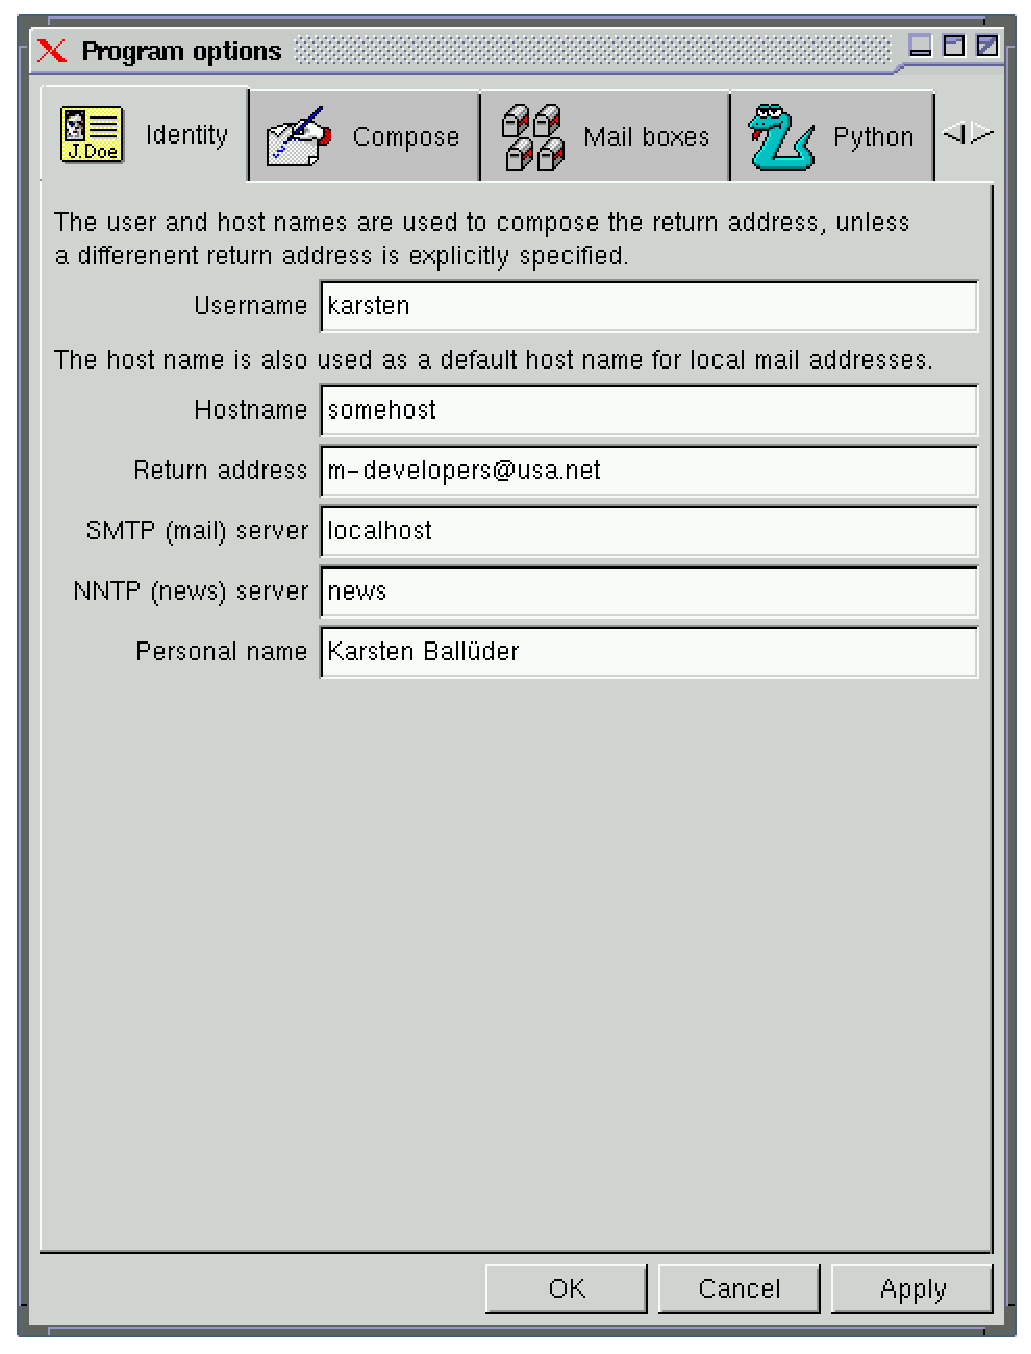
\epsfig{file=pics/Identity.eps}}\end{figure}

Here several important settings are configured, so it is advised (as the program
itself will tell you whenit is run for the first time) to set them up before
starting using M.

\begin{itemize}
\item \textbf{Username}\\
This is used as (default) login name for the accounts which require one (POP3
or IMAP4) and also as the base for the return address unless it is overriden
by explicit setting of the return address.
\item \textbf{Hostname}
\item \textbf{Return address}
\item \textbf{SMTP server}\\
This is the server used for sending outgoing mail, please ask your system administrator
if you don't know its name. If you don't configure this setting, you will not
be able to send any e-mail!
\item \textbf{NNTP server}\\
This is the server used for reading USENET newsgroups.
\item \textbf{Personal name}
\end{itemize}

\subsubsection{Network page}

TODO


\subsubsection{Folders page}

TODO


\subsubsection{Python page}

(only if you have a Python-enabled version of M)

\label{PythonOptions}


\subsubsection{Addressbook page}

M may automatically remember all addresses from all e-mail messages you receive
(actually, only those which you read). This is called \emph{address autocollection}
and, as almost any other feature of M can be turned on and off as desired. In
this page you may choose whether you want to use this feature at all (it is
on by default) and, if so, where should be the autocollected addresses be put
and other settings.

\begin{itemize}
\item \textbf{Autocollect addresses}\\
You may choose ``No'' to disable autollecting addresses completely, or choose
``Yes'' to always autocollect them. The remaining option, ``Ask'', means
that you will be presented with a message box each time an address is about
to be autocollected.
\item \textbf{Address book to use}\\
You may enter the path of the address book to use for autocollected addresses.
Although you may use any address book for this, it is probably better to have
a special address book for all autocollected addresses. If the path name given
here is an absolute one, it is used as is. Otherwise, it is considered to be
relative to your M directory. For example, the default for this option is ``autocollect.adb''
and so the default autocollect book will be created in \noun{\$HOME/.M/autocollect.adb}
under Unix.
\item \textbf{Ignore addresses without names}\\
You may with to autocollect only addresses which have a full name - in this
case you should check this option. If it is off and the address has no name,
the first part of e-mail address (the one preceding the '@' symbol) will be
used instead of the name.
\end{itemize}
In addition to its own built-in addressbook format, M also supports the addressbook
files of the BBDB addressbook used with Emacs (see \ref{BBDB}). Some settings
can be set here which apply only to the BBDB addressbook support:

\begin{itemize}
\item \textbf{Ignore entries without names}\\
BBDB can store entries which have only an e-mail address with them, but no name.
If you set this option, M will discard such entries.
\item \textbf{Generate unique aliases}\\
Setting this option allows M to ensure that all aliases are unique. If two entries
have the same alias, one of them will be modified to distinguish them. This
is especially useful in conjuction with the following option. If this option
is set, reading in of BBDB addressbooks is slowed down considerably. However,
setting it once, then saving the addressbook and disabling it, will make sure
that all aliases are unique without slowing down subsequent loading of the addressbook
the next time it is used.
\item \textbf{Name for nameless entries}\\
If M finds entries without a name and is not set to ignore it, this name will
be used for such entries. It can be combined with the option to generate unique
aliases.
\item \textbf{Save on exit}\\
As saving BBDB addressbook can potentially lead to some loss of information
in the original database file (BBDB and M support different fields), you can
choose whether you want M to automatically save the data on exit or ask you
for confirmation. Read section \ref{BBDB} for more details about how BBDB and
M differ in interpreting the database.
\end{itemize}

\paragraph{Helpers}

On this page you can customise which external helper applications M uses for
different action that it does not perform itself.

\begin{itemize}
\item \textbf{Open URLs with}\\
M will use the program listed here to open URLs embedded in email messages.
If you want to use Lynx as your Web browser you should prefix it with ``xterm
-e'' under Unix in order to open Lynx in a separate window. For example, you
may use \noun{xterm -t Lynx -e Lynx.}
\item \textbf{URL browser is Netscape}\\
If the browser used to open URLs belongs to the family of Netscape programs,
tick this box. Instead of calling a new browser each time, M will tell the already
running Netscape process to load the new URL. Also, don't forget to clear it
if you use another browser - otherwise it will fail to start up.
\item \textbf{Help viewer}\\
The program listed here will be used to view the online help system in HTML
format. Any simple HTML viewer can be used here.
\item \textbf{Help viewer is Netscape}\\
Just like the option for the URL browser, this will take talk to an already
running Netscape process instead of opening a new one each time.
\item \textbf{New Mail Command}\\
The line in this field will be executed whenever M receives new mail. This can
be used to play a sound to notify the user of incoming messages, or do something
else to alert him.
\end{itemize}

\subsubsection{Miscellaneous}

All options which don't fit in any other pages areb collected here.

\begin{itemize}
\item \textbf{Show log window}\\
If this option is on, the log window showing all program messages will be displayed
during program execution. It is advised to leave it on because the log messages
(which can be saved to a file from the log window menu) can be valuable for
the bug reports.
\item \textbf{Splash screen on startup}\\
If this option is on, a splash screen is shown on startup. It will go away when
clicked with the mouse or when a given delay (see the next item) expires.
\item \textbf{Splash screen delay}\\
The delay after which the splash screen disappears.
\item \textbf{Autosave delay}\\
This option allows to automatically save all program settings (but not messages
being composed so far) each time the given delay (in seconds) passes. It can
be disabled by setting the delay to 0, but it is advised to leave it enabled
- so that your changes to the program configuration will be always saved.
\item \textbf{Confirm exit}\\
If this options is on, you will be asked whether you want to leave the program
each time before exiting. The checkbox on the message box with this question
can be used to change the value of this option as well.
\item \textbf{Click folder to open}\\
If this option is on, it is enough to select (for example, by clicking on it)
a folder in the folder tree control in the main window to open it in the integrated
folder view. Double clicking the folder or choosing ``Open'' from the popup
menu will open folder in a separate window. This approach has a drawback of
being a little slow with either very big folders or on slow machines/network
connections, so an alternative way is to uncheck this checkbox. Then double
clicking a folder will be needed to open it in the integrated folder view -
while ``Open'' popup menu item will still open it in a separate window.
\item \textbf{Format for the date}\\
This controls how the dates are shown in the folder view window. The string
here has the same format as an argument to strftime(), on a Unix system you
may execute \noun{man strftime} to see them all.
\item \textbf{Show new mail notification}\\
If this option is on, a message box will be shown each time new messages are
received.
\end{itemize}

\section{The Address Database}


\subsection{Introduction}


\subsection{The native Address Book }


\subsection{Support for BBDB Address Books}

\label{BBDB}M supports reading and writing of BBDB address book files. BBDB
is the Big Brother DataBase used with the Emacs family of editors. If you have
an existing address book file, usually called \texttt{.bbdb}, you can load it
into M and use it. This is especially useful if you have an existing file with
auto-collected email addresses that you want to continue to use.


\paragraph*{Caution:}

The BBDB address book format supports different fields than M's native database.
When reading a BBDB file, M will only read the first two addresses and telephone
numbers and assign them to the ``Home'' and ``Work'' addresses and phone
numbers. All additional addresses and phone numbers, the AKA list and the comments
will get lost. M will only save the information displayed in the address editor
window. Currently saving of phone numbers to BBDB files is unsupported as it
uses a different format from M. \textit{Therefore, reading a BBDB file and saving
it back to disk may lead to a loss of information!}


\chapter{Scripting and Extending \textsl{M}}


\section{Introduction}

\textsl{M} has an embedded Python interpreter, if compiled with Python support
enabled. Python is an object-oriented script language which can be used to write
scripts to be executed by \textsl{M} or even to extend \textsl{M}'s functionality.
Python scripts have full access to all internal M data structures and objects.Scripting
and Python integration A number of user definable callback functions are available.
Scripts have access most objects living in M. Scripting can be disabled in the
Preferences dialog (see \ref{PythonOptions}).

Currently the scripting support is quite basic. If you are interested in writing
scripts and need additional callbacks or support for them within \textsl{M},
please get in touch with the developers who will be happy to add it.


\section{Initialisation }

At startup, \textsl{M} will load a file called \texttt{Minit.py} and call the
\texttt{Minit()} function defined in there, without any arguments.


\section{Callback Functions (Hooks)}

There are a number of callbacks available which will be called from different
places within \textsl{M}. These are defined in the header file \texttt{Mcallbacks.h}.
The documentation of these callbacks can be found in the Classes documentation(\htmladdnormallink{Classes online docs}{classes/index.html}).
All of these callbacks are called with at least two arguments:

\begin{enumerate}
\item The name of the hook for which the function got called, e.g. \texttt{FolderOpenHook}
\item A pointer to the object from which it was called. E.g. for \texttt{FolderOpenHook},
this would be a pointer to a \texttt{MailFolder} object. This object does not
carry a useable type with it and needs to be converted in the callback, e.g.
if the argument is called \texttt{arg} and the object is a \texttt{MailFolder},
the object must either be used as \texttt{MailFolder.MailFolder(arg)} or be
converted as \texttt{mf~=~MailFolder.MailFolder(arg)}. 
\item Some callbacks have a third argument. This is either a single value or a tuple
holding several values.
\end{enumerate}

\section{Namespaces}

To avoid repeatedly typing in the name of the module (\texttt{MailFolder} in
this case), it can be imported into the global namespace with ``\texttt{from~MailFolder~import~{*}}''.
By default modules are not imported into the global namespace and must be explicitly
named.


\section{List of Callbacks}

\vspace{0.3cm}
{\centering \begin{tabular}{|l|c|l|l|l|}
\hline 
Callback Name&
Object Type&
Additional Arguments/Types&
Return Value&
Documentaion\\
\hline 
\hline 
FolderOpenHook&
MailFolder&
&
void&
Called after a folder has been opened.\\
\hline 
FolderUpdateHook&
MailFolder&
&
void&
Called after a folder has been updated.\\
\hline 
FolderSetMessageFlag&
MailFolder&
(long) index of message&
1 if changing flags is ok,0 otherwise&
Called before changing flags for a mesage.\\
&
&
(string)name of flag&
&
\\
\hline 
FolderClearMessageFlag&
MailFolder&
(long) index of message&
1 if changing flags is ok,0 otherwise&
Called before changing flags for a mesage.\\
&
&
(string) name of flag&
&
\\
\hline 
FolderExpungeHook&
MailFolder&
&
1 to expunge, 0 to abort&
Called before expunging messages.\\
\hline 
FolderNewMailHook&
MailFolder&
&
1 to suppress default message, 0 else&
Called when new mail arrived in folder.\\
\hline 
GlobalNewMailHook&
mApplication&
(string) sender of mail&
1 to suppress default message, 0 else&
Called when new mail arrived anywhere.\\
&
&
(string) subject of mail&
&
\\
\hline 
\end{tabular}\par}
\vspace{0.3cm}


\section{Supported Classes}

Python has access to M's internal class hierarchy. At present we supply interface
definitions and Python modules for only a small number of classes, however if
there is need for more classes being supported, we can easily extend the list
- please ask us if you want more support!

Some automatically generated documentation of the Python interface to M classes
can be found in the \htmladdnormallink{doc/Python directory}{../Python/}. Documentation
about all classes, including those not available to Python, can be found in
the \htmladdnormallink{doc/classes directory}{../classes/}.


\chapter{Getting Help and Support}


\section{WWW Support}

M has a home on the world wide web where you can get up to date information
about development and the last releases. Come and visit us at the \htmladdnormallink{M Homepage}{http://www.phy.hw.ac.uk/~karsten/M/}


\section{Mailing Lists}

Currently there exist three different mailing lists to help support M users:


\paragraph{m-announce:}

\begin{itemize}
\item M-announce is a moderated list which distributes announcements of new releases
of M. It is a low volume mailing list.
\item To subscribe send an e-mail to: \htmladdnormallink{m-announce-subscribe@egroups.com}{mailto:m-announce-subscribe@egroups.com}
\item To unsubscribe send an e-mail to: \htmladdnormallink{m-announce-unsubscribe@egroups.com}{mailto:m-announce-unsubscribe@egroups.com}
\end{itemize}

\paragraph*{m-users:}

\begin{itemize}
\item M-Users is an unmoderated list for users of M to discuss problems and enhancements.
All announcements will be sent to this list, too. It carries any kind of general
discussion about M. If you just have simple questions which might not constitute
a real bug report, try asking for help on m-users.
\item To subscribe send an e-mail to: \htmladdnormallink{m-users-subscribe@egroups.com}{mailto:m-users-subscribe@egroups.com}
\item To unsubscribe send an e-mail to: \htmladdnormallink{m-users-unsubscribe@egroups.com}{mailto:m-users-unsubscribe@egroups.com}
\end{itemize}

\paragraph*{m-developers:}

\begin{itemize}
\item M-developers is a moderated mailing list for the people involved in M's development
and testing. There are generally two reasons why you would want to send an e-mail
here: \htmladdnormallink{m-developers@egroups.com}{mailto:m-developers@egroups.com}

\begin{enumerate}
\item You have discovered a bug or problem in M and want to tell the developers about,
or, even better, you want to submit a patch to fix it.
\item You want to help develop, translate or test M. This is highly welcome and encouraged.
Please, if you want to add a feature, get in touch with us.
\end{enumerate}
\item If you want to contact the developers, send an e-mail to the address above.
\item Subscription to this list is by invitation only. If you would like to join the
team, contact the developers and we will be happy to add you to the list.
\end{itemize}

\paragraph{Subscribe Directly}

If your help browser understands HTML forms, you will find to forms below where
you can directly subscribe to the support mailing lists.

\begin{rawhtml}<form method=GET action="http://www.findmail.com/cgi-bin/subscribe.py"><input  type=hidden name="listname" value="m-announce"><table BORDER=0 CELLSPACING=0 BGCOLOR="#000000" ><tr><td><table BORDER=0 CELLSPACING=0 CELLPADDING=3 WIDTH="300" BGCOLOR="#FFFFCC" ><tr><td ALIGN=CENTER BGCOLOR="#000000"><b><fontface="arial,helvetica"><font color="#FFFFFF">Subscribe to M-announcements list&nbsp;</font></font></b></td></tr><tr><td>Enter your e-mail address:&nbsp;</td></tr><tr><td><input type=text name="emailaddr" value="your e-mail" size=21><input type=submit name="SubmitAction" VALUE="Subscribe"></td></tr><tr><td><a href="http://www.findmail.com/list/m-annouce/">FindMail List Archive</a></td></tr><tr><td><font face="arial,helvetica"><font size=-1>A mailing list hosted by<a href="http://www.makelist.com/">MakeList!</a></font></font></td></tr></table></td></tr></table> </form>\end{rawhtml}

\begin{rawhtml}<form method=GET action="http://www.findmail.com/cgi-bin/subscribe.py"><input  type=hidden name="listname" value="m-users BORDER=0 CELLSPACING=0 BGCOLOR="#000000" ><tr><td><table BORDER=0 CELLSPACING=0 CELLPADDING=3 WIDTH="300" BGCOLOR="#FFFFCC" ><tr><td ALIGN=CENTER BGCOLOR="#000000"><b><fontface="arial,helvetica"><font color="#FFFFFF">Subscribe to M-users forum&nbsp;</font></font></b></td></tr><tr><td>Enter your e-mail address:&nbsp;</td></tr><tr><td><input type=text name="emailaddr" value="your e-mail" size=21><input type=submit name="SubmitAction" VALUE="Subscribe"></td></tr><tr><td><a href="http://www.findmail.com/list/m-annouce/">FindMail List Archive</a></td></tr><tr><td><font face="arial,helvetica"><font size=-1>A mailing list hosted by<a href="http://www.makelist.com/">MakeList!</a></font></font></td></tr></table></td></tr></table> </form>\end{rawhtml}

If there are no forms above this line, you need to subscribe by email or visit
the \htmladdnormallink{M Homepage}{http://www.phy.hw.ac.uk/~karsten/M/}


\subsection*{Mailing List Archives}

All three mailing lists are archived at \htmladdnormallink{Egroups.com}{http://www.egroups.com/}


\chapter{Compiling \textsl{M} from source}

These compilation notes are probably a bit outdated. The best start is to use
the \texttt{-{}-help} option of configure to see which options it supports.


\section{General Procedure}


\subsection{Prerequisites}

Before you can compile M, you will need a matching copy of \htmladdnormallink{wxWindows}{http://web.ukonline.co.uk/julian.smart/wxwin/},
that is, if compiling under Unix, you will need \htmladdnormallink{wxGTK}{http://www.freiburg.linux.de/~wxxt/}.
As wxGTK is under constant development, you should use the same copy of wxGTK
that we used to build M, you can get it from the \htmladdnormallink{M download page}{http://www.phy.hw.ac.uk/~karsten/M/download.html}.


\subsection{Configuring wxGTK}


\subsubsection{Unpack wxGTK and run its \texttt{configure} script:}

\begin{quote}
\texttt{./configure~-{}-without-threads~-{}-with-gtk~-{}-without-shared~-{}-without-debug\_flags
}~\\
~\texttt{-{}-without-debug\_info~-{}-without-odbc}
\end{quote}
Of course, feel free to change the two debug options to \texttt{-{}-with-debug}
if you want to generate a version with debugging enabled.


\subsubsection{Compile and install wxGTK}

Change into the src directory and run \texttt{make} and \texttt{make~install}.
wxGTK requires libgtk 1.0.x, it does not work with gtk-1.1 (yet).


\subsection{Configuring M}

As with wxGTK, just run M's \texttt{configure} script. If you have built wxGTK
with debugging enabled, specify the additional option \texttt{-{}-with-debug}
when configuring M. Call \texttt{./configure~-{}-help} to get a list of supported
options. Generally you will just run it without options. If configure fails
to find some header files or libraries, you can create links to them in the
\texttt{extra/include} and \texttt{extra/lib} directories and configure will
find them. To reconfigure M, make sure that you delete any \texttt{{*}cache{*}}
files first.


\subsection{Compiling M}

Just run \texttt{make} from the top level M directory. If you later want to
rebuild M without rebuilding the libraries contained in the \texttt{extra/src}
directory, i.e. after changing the M source, just run \texttt{make} in the \texttt{src}
directory.


\subsubsection{To generate the documentation}

...type \texttt{make~doc} from the main directory or simply \texttt{make} in
the doc directory.


\subsection{Installing M}

Just call any or all of the following make targets in the main directory:


\subsubsection{make install}

Will compile and install M and the required additional files.


\subsubsection{make install\_doc}

Will install and, if necessary, regenerate the documentation and online help
system.


\subsubsection{make install\_locale}

Will attempt to generate message catalogs for translations and install them.
Note that M is not fully translated yet.


\subsubsection{make install\_all}

Will do all of the above


\subsection{Some extra software might be required}

For regenerating the documentation you will need \texttt{doc++} for generating
the class documentation. Alternatively the Makefile system will try to use kdoc
or scandoc (included), but might fail halfway during class documentation generation.
Also, latex, latex2html, netpbm and plenty of disk space on \texttt{/tmp} are
required for generating the online docs. However, the distribution includes
a file Mdoc.tar.gz in the doc directory. As long as you leave this file there,
the Makefile will not attempt to regenerate the documentation but use this instead.


\section{Operating systems specific}


\subsection{Linux}

If compiling with a non-default compiler like \texttt{egcs}, make sure that
\texttt{/usr/include} is not in the include path, neither should \texttt{/usr/lib}
be explicitly listed. M has been compiled with \texttt{egcs} and \texttt{gcc-2.8.x}
on both, \texttt{libc5} and \texttt{glibc2} systems.


\subsection{Solaris/SunOS}

M has been successfully compiled with \texttt{gcc-2.8.0} on Solaris. Currently
it does not compile with the standard \texttt{C++} compiler.


\subsection{Microsoft Windows }

M can be compiled under Windows, using wxWindows Version 2.0 and Microsoft Visual
C++ version 4.x or later. The makefiles are included in the M source distribution
(they will build the version of M without Python support).


\subsection{DEC Alpha with Digital UNIX 3.2c}

(Karsten Ball�der: It seemed at that time that the segmentation fault was caused
by a bug in wxGTK. By now this should be fixed. However, no new attempt to compile
M on DEC Unix has been made yet. However, I include Holger's report as a help
for some future attemp.)

This section has been contributed by Holger Bauer 
\texttt{\small \htmladdnormallink{bauer@itsm.uni-stuttgart.de}{bauer@itsm.uni-stuttgart.de}
\htmladdnormallink{http://www.itsm.uni-stuttgart.de/~bauer}{http://www.itsm.uni-stuttgart.de/~bauer}}{\small \par}

\begin{enumerate}
\item First I took the following arguments for configure:\\
\texttt{\small configure~-{}-x-includes=/usr/X11R6/include~-{}-x-libraries=/usr/X11R6/shlib
-{}-with-wxGTK~-{}-without-python}~\\
{\small This would not work since}~\texttt{\small make~dep} {\small still tries
to find}~\texttt{\small Python.h}{\small .}\\
{\small Therefore I created a dummy include file Python.h in}\texttt{\small  \dots/M/src/Python}{\small .
This helped to complete make dep. \label{item1}}{\small \par}
\item However step \ref{item1} still reported some warnings:\\
\texttt{\dots/M/extra/src/c-client/mail.h} would complain about a missing \texttt{linkage.h}
header file. Also, a missing \texttt{osdep.h} file was reported.\\
\texttt{\dots/M/extra/src/c-client/osdep.h} falsely pointed to \texttt{os\_gof.h}
but this file was missing. Therefore copied~\texttt{os\_osf.h} to~\texttt{os\_gof.h}.
Also, copied~\texttt{os\_osf.c} to~\texttt{os\_gof.c} since \texttt{osdepbas.c}
pointed to~\texttt{os\_gof.c}. 
\item \texttt{cd~src;}~\\
\texttt{make;}\\
This would fail since swig was not searched for by the configure script. Since
even I gave --without-python to configure make would search in /src/Python and
try to compile things there I decided to install python and swig.
\item The Python-FAQ states that python definitely has to be compiled with the DEC
cc.
\item After that I took:\\
\texttt{\small configure~-{}-x-includes=/usr/X11R6/include~-{}-x-libraries=/usr/X11R6/shlib
-{}-with-wxGTK}~\\
{\small The make process would then stop in}\texttt{ \dots/M/src/adb/AdbFrame.cpp}.
The line 
\texttt{AdbTreeElement~{*}current~=~wxIsPathSeparator(strEntry{[}0u{]})\dots
}would not compile since the wxString function takes a long integer (due to
the 64 bit architecture).\\
This error might disappear if somebody adjusts the wxString library accordingly.\\
In meantime (for my local \texttt{libwx\_gtk.so}) I changed to \texttt{strEntry{[}0{]}}.
\item Then only final linkage errors occured:\\
\texttt{-lpthread} is not known, needs \texttt{-lpthreads}\\
\texttt{-lcrypt} is not known, just omit\\
\texttt{-ldmalloc} is not known, pass~\texttt{-{}-without-dmalloc} to~\texttt{configure}.
\item Because the link process did not give me any error I expected M to run (at least
some kind of unstable). But a core dump appeared immediately.\\
\texttt{dbx} gives to following information:\\
\texttt{(dbx)~run~}~\\
\texttt{signal~Segmentation~fault~at~>{*}{[}mig\_get\_reply\_port,~0x3ff83004a0c{]}
stq~r26,~0(sp)~}~\\
\texttt{(dbx)~where~}~\\
\texttt{>~0~mig\_get\_reply\_port(0xffffffffffffffff,~0xffffffffffffffff,~0xffffffffffffffff,
0xffffffffffffffff,~0xffffffffffffffff)~{[}0x3ff83004a0c{]}~}~\\
The output of \texttt{gdb} is not very appealing:\\
\texttt{(gdb)~run~Starting~program:~/usr3/bauer/src/M/M/src/M~}~\\
\texttt{Program~received~signal~SIGSEGV,~}~\\
\texttt{Segmentation~fault.~0x3ff83008f5c~in~port\_allocate~()}~\\
\texttt{(gdb)~where}~\\
\texttt{\#0~0x3ff83008f5c~in~port\_allocate~()~\#1~0x3ff83004a38~in~mig\_get\_reply\_port
()~}~\\
\texttt{\#2~0x3ff83008f94~in~port\_allocate~()~\#3~0x3ff83004a38~in~mig\_get\_reply\_port
()}~\\
This output runs until infinity \dots.
\end{enumerate}

\section{Configuration and Testing}

Under Unix all configuration settings are stored in \texttt{\~{}/.M/config}
under Windows in the registry. To get an overview over all possible configuration
options and their default values, set the value \texttt{RecordDefaults=1}. Under
Unix, do this by creating a new \texttt{\~{}/.M/config} file containig the lines

\verb|[M]|

\verb|RecordDefaults=1|

After running M, this file will then contain all default settings. Most of them
are easily understood. Otherwise, the file \texttt{include/Mdefaults.h} contains
them all with some short comments.


\section{wxWindows}

You will need the wxWindows GUI toolkit to compile \textsl{M}.

Further Information

\begin{itemize}
\item wxWindows is available from \texttt{http://web.ukonline.co.uk/julian.smart/}
\item The GTK port of wxWindows, wxGTK, is available from: http://www.freiburg.linux.de/\~{}wxxt/
\end{itemize}
In order to compile this alpha release of \emph{M} you will need wxWindows 2.0
strictly later than beta 3 and so it is probably easier to take the wxWindows
sources snapshot from the \emph{M} home page.


\chapter{FAQ - Frequently Asked Questions}

Being a brand new program, this section is currently empty. However, we will
constantly update this chapter with questions received on the mailing lists.

\end{document}
